\documentclass[a4paper,12pt]{article}
\usepackage{graphicx} % Required for inserting images
\usepackage{color}
\usepackage[UTF8]{ctex}
\usepackage{amsmath}
\usepackage{tabularray}



%\newcommand{\upsite}[1]{\textsuperscript}{cite{#1}}

%\bibliographystyle{unsrt}
\begin{document}
\begin{figure}[t]
    
\includegraphics[width=0.2\textwidth]{ouc.jpg}
\end{figure}

\title{实验报告}
\author{单衍喆 }
\date{2024-9-12}
\maketitle

\pagenumbering{roman}
\text{GitHub地址:https://github.com/Venusss1/course.git}
\tableofcontents
\newpage
%\pagenumbering{arabic}


\section{\underline{\color{blue}实验内容}}

\begin{enumerate}
    \item \textbf{python基础}
    \item \textbf{pytorch图像处理基础}
\end{enumerate}

\section{\underline{\color{blue}实验设计}}
\subsection{\color{red}python基础}

\subsubsection{\color{green}python简介}

\begin{itemize}
    \item python是解释型语言:开发过程中没有编译环节
    \item python是交互式语言:可以再python提示符>>>后直接执行代码
    \item python是面向对象语言:支持面向对象的风格和代码封装
    \item python对初学者友好:便于学习且应用广泛
\end{itemize}

\subsubsection{\color{green}python环境配置}
\begin{enumerate}
    \item 下载安装python
          \begin{figure}[htbp]
              \centering
              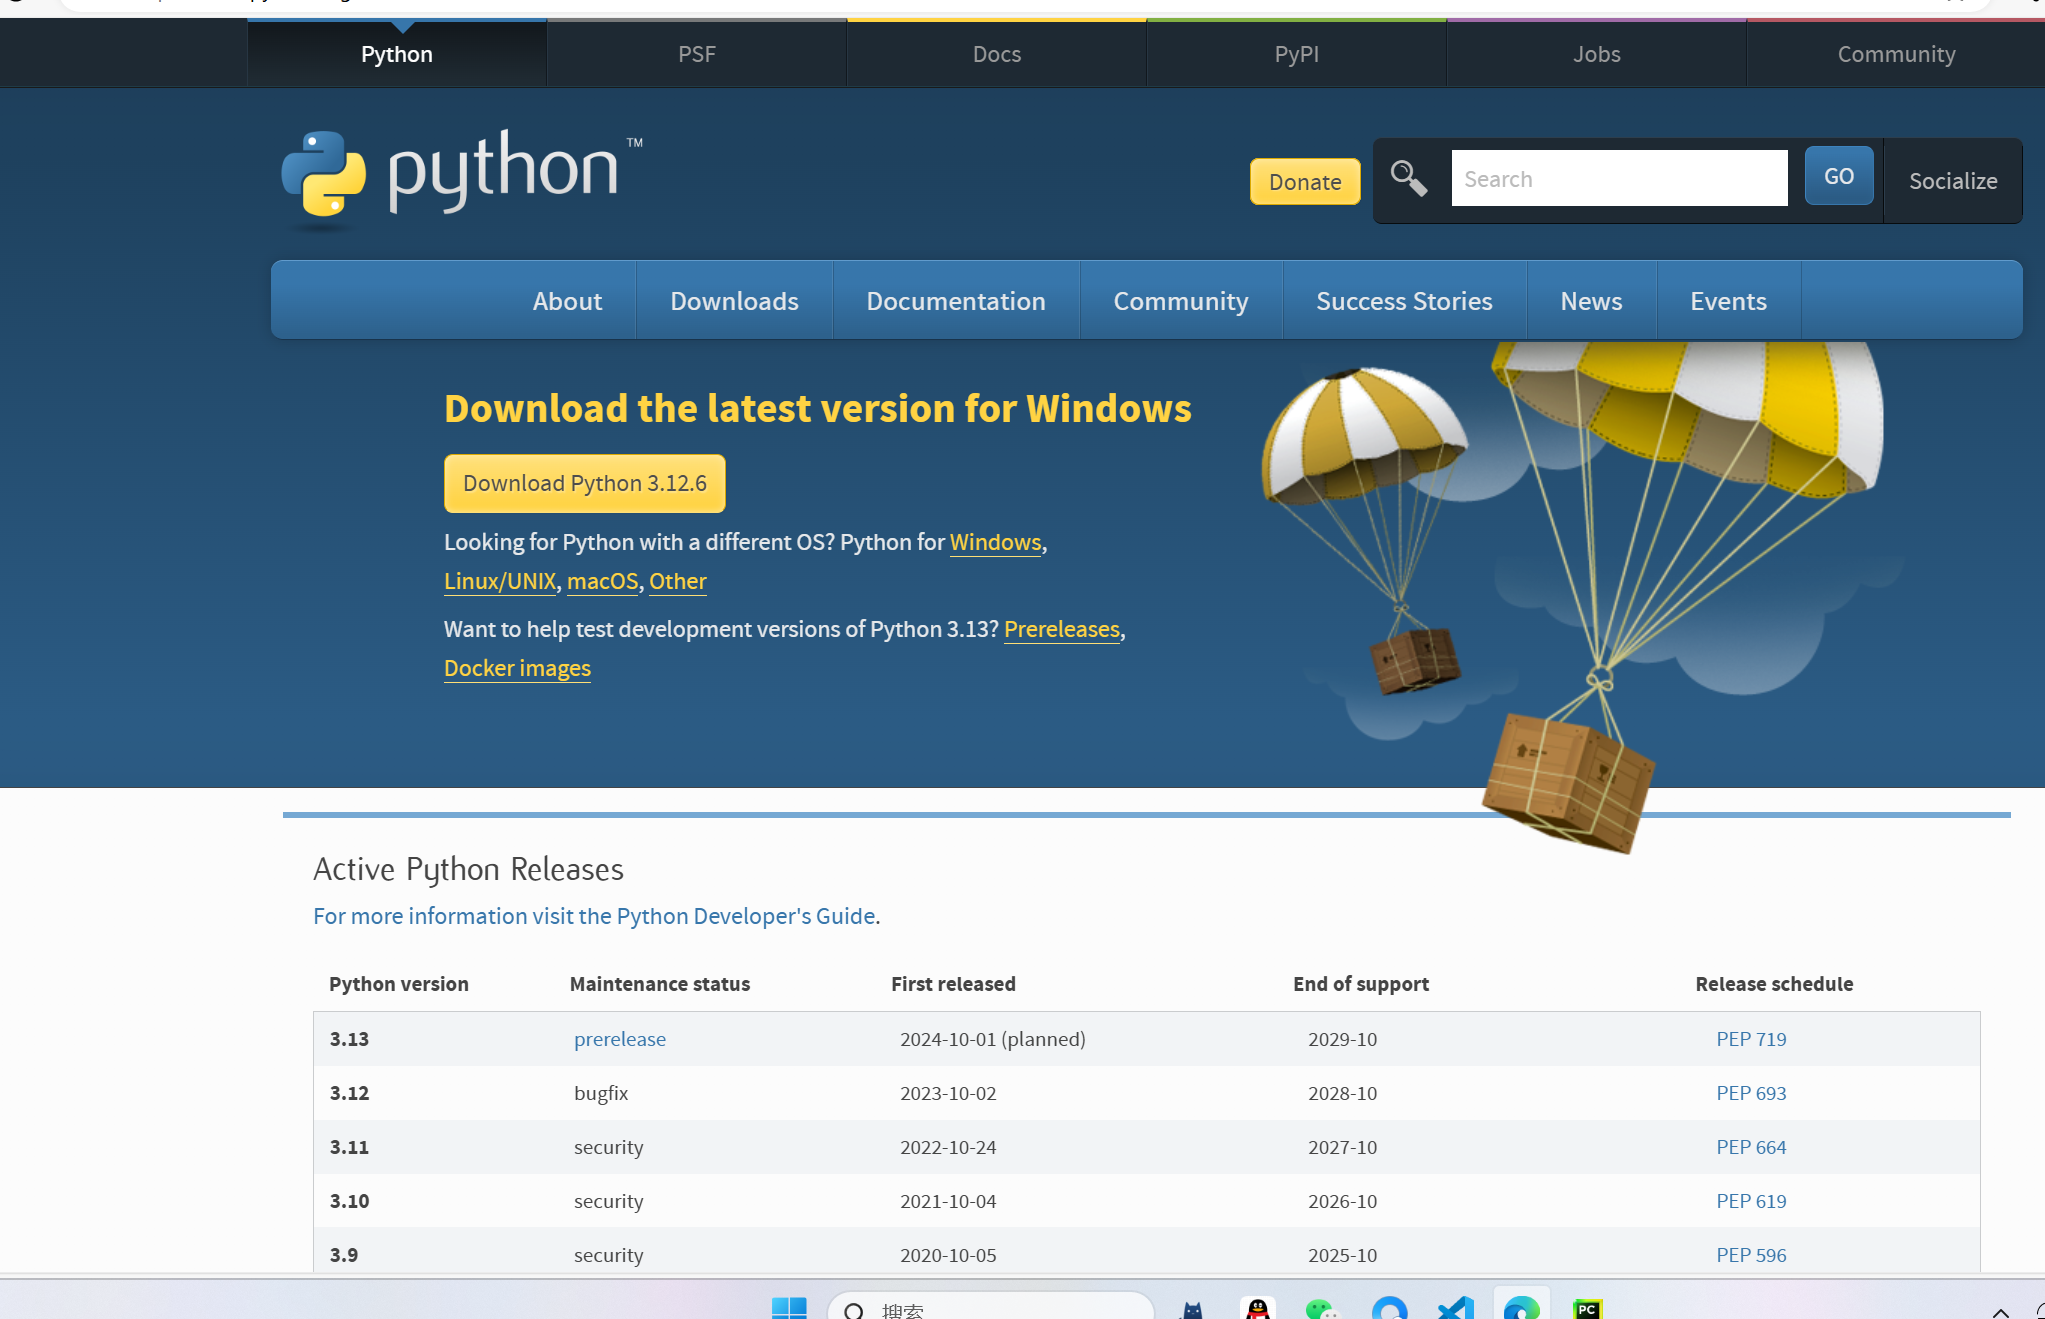
\includegraphics[width=0.5\textwidth]{install.png}
              \caption{python官网}
          \end{figure}
    \item 配置环境变量
         \begin{figure}[htbp]
              \centering
              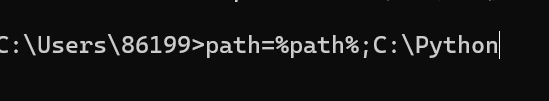
\includegraphics[width=0.5\textwidth]{path.png}
              \caption{环境变量配置}
          \end{figure}
    \item 安装pycharm
\end{enumerate}
\subsubsection{\color{green}python与c的语法差异}

\definecolor{MineShaft}{rgb}{0.2,0.2,0.2}
\begin{table}[h]
\centering
\caption{语法差异}
\begin{tblr}{
  cell{1}{2} = {c},
  cell{1}{3} = {c},
  cell{2}{1} = {c},
  cell{2}{2} = {fg=MineShaft},
  cell{2}{3} = {fg=MineShaft},
  cell{3}{1} = {c},
  cell{3}{2} = {fg=MineShaft},
  cell{4}{1} = {c},
  cell{4}{2} = {fg=MineShaft},
  cell{4}{3} = {b},
  vline{2-3} = {-}{},
  hline{1-2} = {-}{},
}
差异  & python                                       & c                                   \\
缩进  & 用缩进来写模块                                      & 使用大括号~\textbf{\{\}}~来控制类,函数以及其他逻辑判断 \\
结束符 & 一般以新行作为语句的结束符                                & 使用';'作为语句结束                         \\
引号  & 可以使用引号(~'~)、双引号(~"~)、三引号(~'''~或~"""~) 来表示字符串 & 单引号和双引号分别表示单个字符和字符串                 
\end{tblr}
\end{table}


\newpage
\subsubsection{\color{green}循环}
python提供了for循环和while循环(没有do...while循环)
\begin{figure}[h]
    \centering
    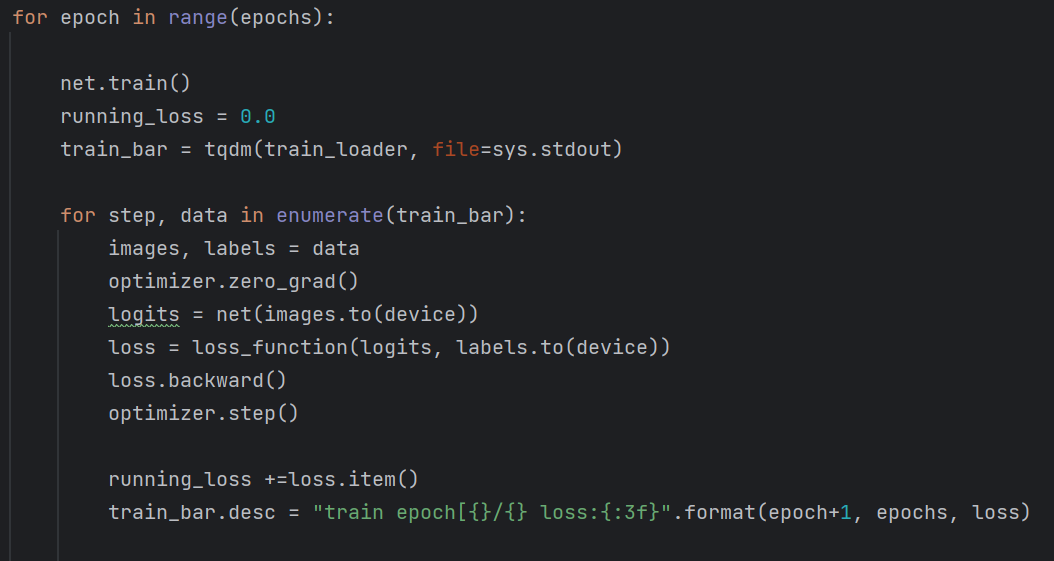
\includegraphics[width=0.5\textwidth]{for.png}
    \caption{for循环}
\end{figure}
\subsubsection{\color{green}数据类型}
python主要的数据类型:字符串,列表,元组,字典

\begin{figure}[h]
    \centering
    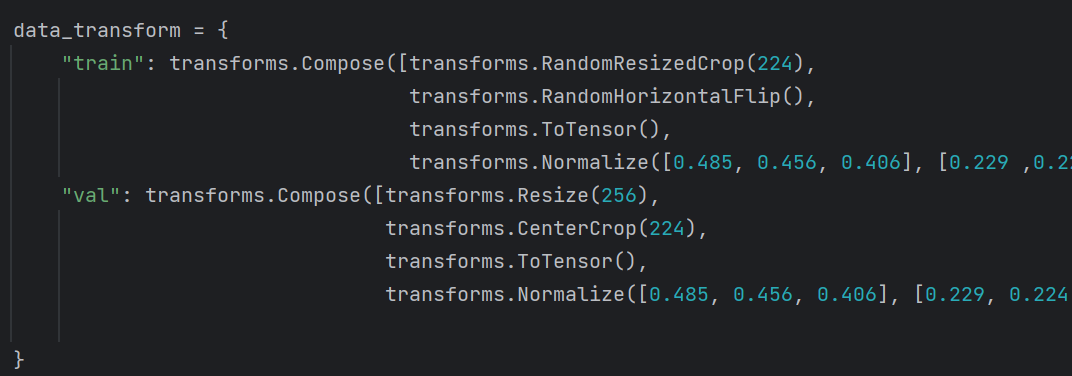
\includegraphics[width=0.5\textwidth]{dict.png}
    \caption{字典(键值对)}
\end{figure}





\subsection{\color{red}pytorch视觉应用}

\subsubsection{\color{green}PIL:python图像处理类库}
PIL提供通用图像处理功能:缩放,裁剪,旋转,颜色转换
\begin{itemize}
    \item 读取图像:
            \begin{verbatim}
            from PIL import Image
            pil_im = Image.open('empire.jpg')
            \end{verbatim}
    \item 颜色转换
            \begin{verbatim}
            pil_im = Image.open('empire.jpg').convert('L')
            \end{verbatim}
    \item 图像保存
            \begin{verbatim}
            Image.open(infile).save(outfile)
            \end{verbatim}
    \item 创建缩略图
            \begin{verbatim}
            pil_im.thumbnail((128,128))
            \end{verbatim}
    \item 复制和粘贴图像区域
            \begin{verbatim}
            box = (100,100,400,400)
            region = pil_im.crop(box)
            pil_im.paste(region,box)
            \end{verbatim}
    \item 调整尺寸
            \begin{verbatim}
            pil_im.resize((128,128))
            \end{verbatim}
    \item 旋转
            \begin{verbatim}
            pil_im.rotate(45)
            \end{verbatim}
\end{itemize}

\subsubsection{\color{green}Matplotlib}

\begin{itemize}
    \item 绘制图像、点和线
            \begin{enumerate}
                \item 导入模块
                    \begin{verbatim}
                    from pylab import *
                    x = [100,100,400,400]
                    \end{verbatim}
                \item 绘制点
                    \begin{verbatim}
                    plot(x,y,'r*')
                    \end{verbatim}
                \item 绘制线
                    \begin{verbatim}
                    plot(x[:2],y[:2])
                    \end{verbatim}
                \item 显示图像
                    \begin{verbatim}
                    imshow(im)
                    \end{verbatim}
            \end{enumerate}
    \item 图像轮廓和直方图
        \begin{verbatim}
        图像轮廓
            figure()
            gray()
            contour(im,origin='image')
        直方图
            figure()
            hist(im.flatten(),128)
            show()
        \end{verbatim}
    \item 交互
       \begin{verbatim}
         x = ginput(3)
       \end{verbatim}
        
\end{itemize}

\subsubsection{\color{green}NumPy}
NumPy帮助实现数组中的操作
\begin{itemize}
    \item 图像数组表示
        \begin{verbatim}
        im = array(Image.open('empire.jpg').convert('L','f'))
        \end{verbatim}
    \item 灰度变换
        \begin{verbatim}
        im2 = 255 - im
        im3 =(100.0/255)*im + 100
        im4 = 255.0*(im/255.0)**2
        \end{verbatim}
    \item 图像缩放
        \begin{verbatim}
        def imresize(im,sz):
            pil_im = Image.fromarray(uint8(im))
            return array(pil_im.resize(sz))
        \end{verbatim}
    \item 主成分分析
        \begin{verbatim}
        def pca(X):
           num_data,dim = X.shape
           mean_X = X.mean(axis=0)
           X = X - mean_X
           ...
           return V,S,mean_X
        \end{verbatim}
\end{itemize}

\subsubsection{\color{green}SciPy}
SciPy建立于NumPy基础上,用于数值计算
\begin{itemize}
    \item 图像模糊
        \begin{verbatim}
        使用scipy.ndimage.filters模块计算卷积
        from scipy.ndimage import filters
        im2 = filters.gaussian_filter(im,5)
        模糊彩色图像只需对每一个颜色通道进行高斯模糊
        \end{verbatim}
    \item 图像导数
        \begin{verbatim}
        sobel导数滤波器
        filters.sobel(im,2,imx)
        magnitude = sqrt(imx**2+imy**2)
        \end{verbatim}
\end{itemize}

\newpage
\section{\underline{\color{blue}实验心得}}
通过本次实验,我学会了python的基础语法,安装了pycharm并在本地配置完成了python环境
我学会了pytorch处理图像的基本方法,了解了pytorch处理图像的常用库及对应方法


\end{document}
